\begin{figure}[h!]
    \centering
    \caption{Probability of being a renter by household income decile,
    full sample}
    \label{fig:ahs_pr_renters}

    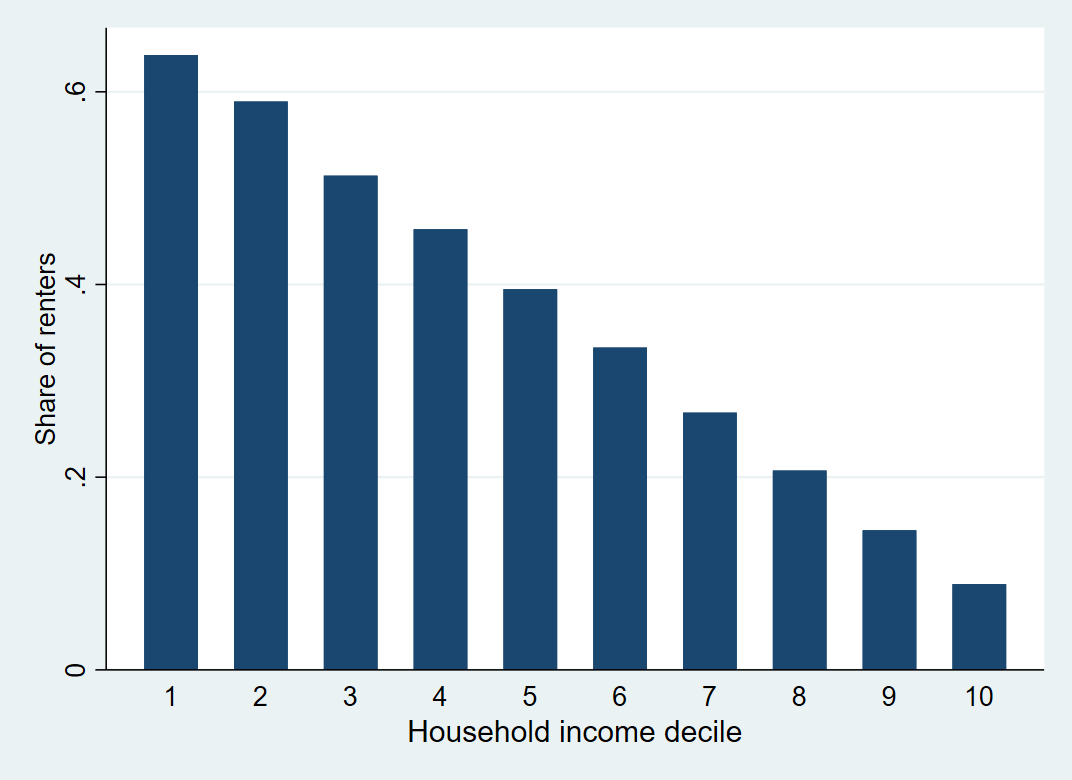
\includegraphics[width = 0.75\textwidth]{ahs/output/sh_renters.png}

    \begin{minipage}{.95\textwidth} \footnotesize
        \vspace{3mm}
        Notes: Data are from the 2011 and 2013 American Housing
        Survey \parencite{ahs2020}, as described in 
        Section XX. 
        The figure shows the probability of a household being
        rented by household income. 
        We construct hte figure as follows: first, we residualize an
        indicator for being a renter and household income by SMSA,
        a concept of metropolitan areas available in the data.
        Second, we construct deciles of the residualized household
        income variable.
        Finally, we take the average of the residualized renter 
        indicator within each decile.
        We exclude from the calculation non-conventional housing units, 
        such as mobile homes, hotels, and others.
    \end{minipage}
\end{figure}
